\documentclass[12pt]{article}

\usepackage[utf8]{inputenc}

\usepackage{mathpazo}
\usepackage{domitian}


\usepackage[T1, T2A]{fontenc}
\usepackage[russian]{babel}
\let\oldstylenums\oldstyle

\usepackage{amssymb,amsmath,mathrsfs,amsthm}

\usepackage{needspace}
\usepackage{wrapfig}
\usepackage{subcaption}
\usepackage{graphicx}
\usepackage[colorlinks,linkcolor=black,citecolor=black, unicode]{hyperref}
\usepackage{indentfirst}

% Параметры страницы
\textheight=24cm % высота текста
\textwidth=16cm % ширина текста
\oddsidemargin=0pt % отступ от левого края
\topmargin=-2.5cm % отступ от верхнего края
\parindent=15pt % абзацный отступ
\parskip=5pt % интервал между абзацам
\tolerance=2000 % терпимость к "жидким" строкам
\flushbottom % выравнивание высоты страницa
\renewcommand{\baselinestretch}{1.1}

%math operations
\newcommand{\norm}{\mathop{\rm norm}\limits}
\newcommand{\real}{\mathbb{R}}
\newcommand{\ex}{\mathbb{E}}
\newcommand{\diag}{\mathrm{diag}}
\newcommand{\intset}{\mathrm{int}}
\newcommand{\softmax}{\mathop{\rm softmax}\limits}
\newcommand{\lossfunc}{\mathcal{L}'}
\newcommand{\elbo}{\mathcal{L}}
\newcommand{\normal}[3]{\mathcal{N}(#1 | #2, #3)}
\newcommand{\dd}[2]{\frac{\partial#1}{\partial#2}}
\newcommand{\kl}[2]{\mathop{KL}(#1 \parallel #2)}
\newcommand{\nm}{\mathcal{N}}
\newcommand{\sle}{\; \Rightarrow \;}
\newcommand{\indpos}{\mathbf{I}_{d_k}^{+}[i, j]}
\newcommand{\indneg}{\mathbf{I}_{d_k}^{-}[i, j]}

%my settings
\graphicspath{{../figures/}}

\begin{document}

\begin{titlepage}
    \begin{center}
        Московский государственный университет имени М. В. Ломоносова
    
        \bigskip
        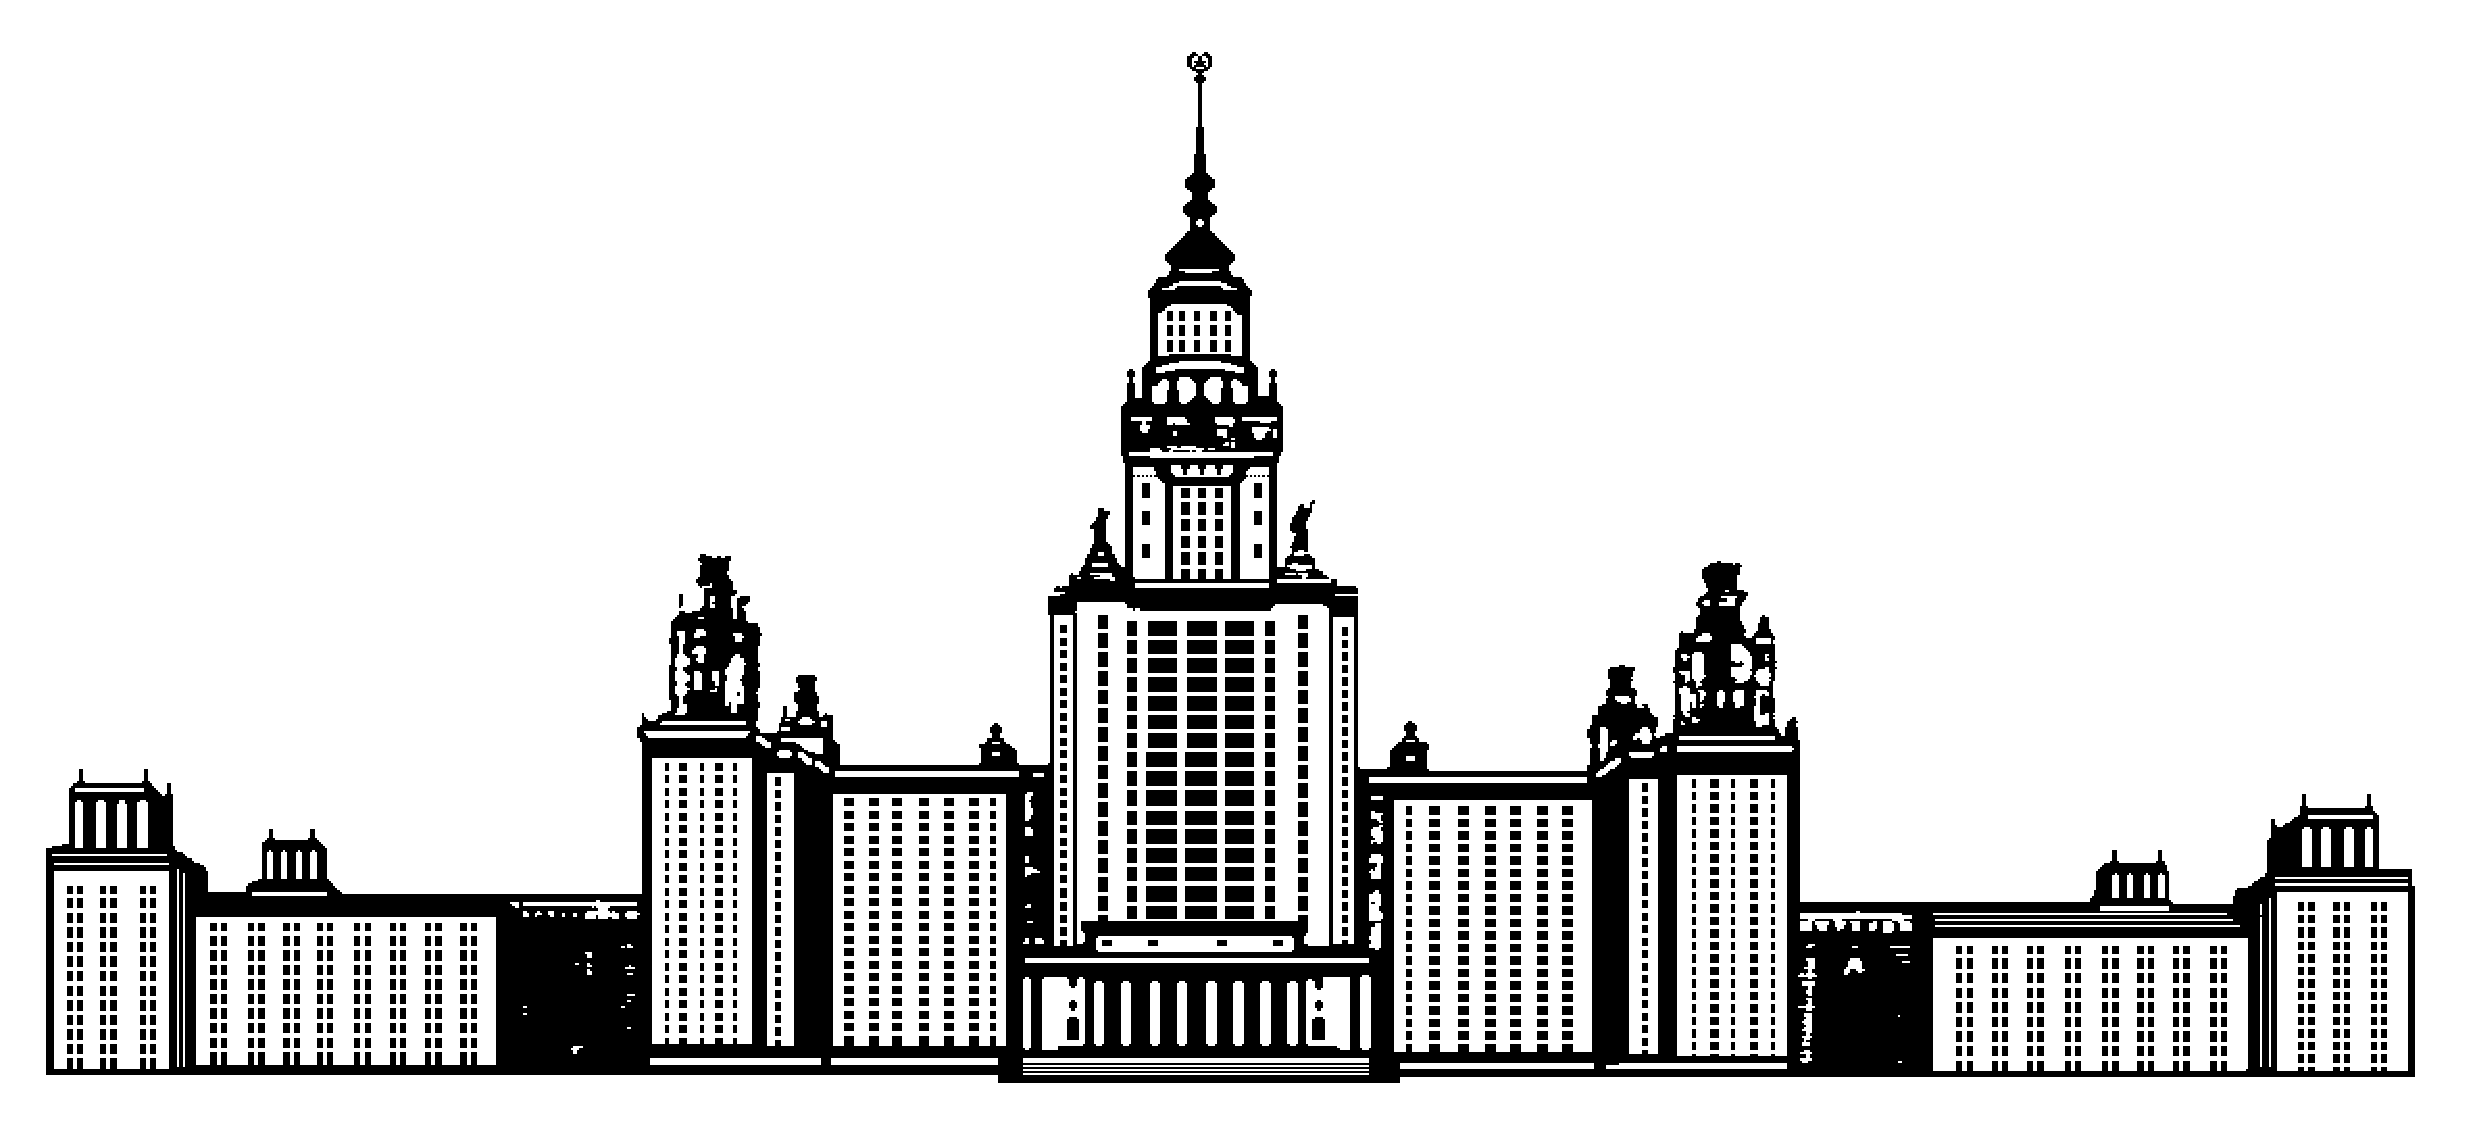
\includegraphics[width=50mm]{msu.pdf}
    
        \bigskip
        Факультет Вычислительной Математики и Кибернетики\\
        Кафедра Математических Методов Прогнозирования\\[10mm]
    
        {\large\bfseries
            ОТЧЕТ О ПРЕДДИПЛОМНОЙ ПРАКТИКЕ СТУДЕНТА 417 ГРУППЫ\\[10mm]
            ''Распознавание и генерация изображений рукописных текстов на русском языке''}
        \\[100mm]
        
    
        \begin{flushright}
            \parbox{0.4\textwidth}{
                Выполнил:\\
                студент 4 курса 417 группы\\
                \emph{Тыцкий Владислав Игоревич}
            }
        \end{flushright}
    
        \vspace{\fill}
        Москва, 2021
    \end{center}
\end{titlepage}


\section*{Аннотация}
Распознавание текста (Optical Character recognition) одна из известных задач в области машинного обучения.
Много лет люди хорошо решают эту задачу для печатных текстов, но в то же время в распознавании рукописных текстов
возникает за собой много трудностей, которые сложно решить. В данном отчете будет будет описан сбор датасета,
обучение модели распознавания, а также генерация синтетического датасета с помощью GAN (Generative Adversarial Network)

\newpage

\tableofcontents

\newpage

\section{Введение}
Распознавание текста (Optical Character recognition) одна из известных задач в области машинного обучения.
Много лет люди хорошо решают эту задачу для печатных текстов, но в то же время распознавание рукописных текстов
влечет за собой много трудностей, которые нужно решать.
Одна из проблем -- это малое количество данных для обучения. Сбор датасета с рукописными текстами
времязатратен и дорог, помимо этого получение изображений текста  лишь первый этап, за которым следует обработка и разметка данных.
Вторая проблема -- высокая сложность генерации синтетических данных. В отличии от рукописных данных,
печатные тексты несложно сгенерировать: выбираем шрифт, пишем определенный текст и подставляем его на белый фон. Даже такие простые
манипуляции могут давать данные, на которых можно обучить работающую модель распознавания.

\subsection{Данные}
На сегодняший день известно не так много датасетов с рукописными текстами. 

\vspace{10pt}

Некоторые из них:
\begin{itemize}
    \item IAM database \cite{iam} -- датасет английских рукописных текстов
    \item RIMES database -- датасет французских рукописных текстов
    \item Cyrillic Handwriting Dataset (CyrHD)  \cite{chd} -- датасет русских рукописных текстов \textit{(преимущественно слов)}
    \item Handwritten Kazakh and Russian (HKR)  \cite{hkr} -- датасет русских/казахских рукописных текстов \textit{(не для коммерческого использования)}
\end{itemize}


\subsection{Модели распознавания}

\begin{figure}[htb]
    \centering
    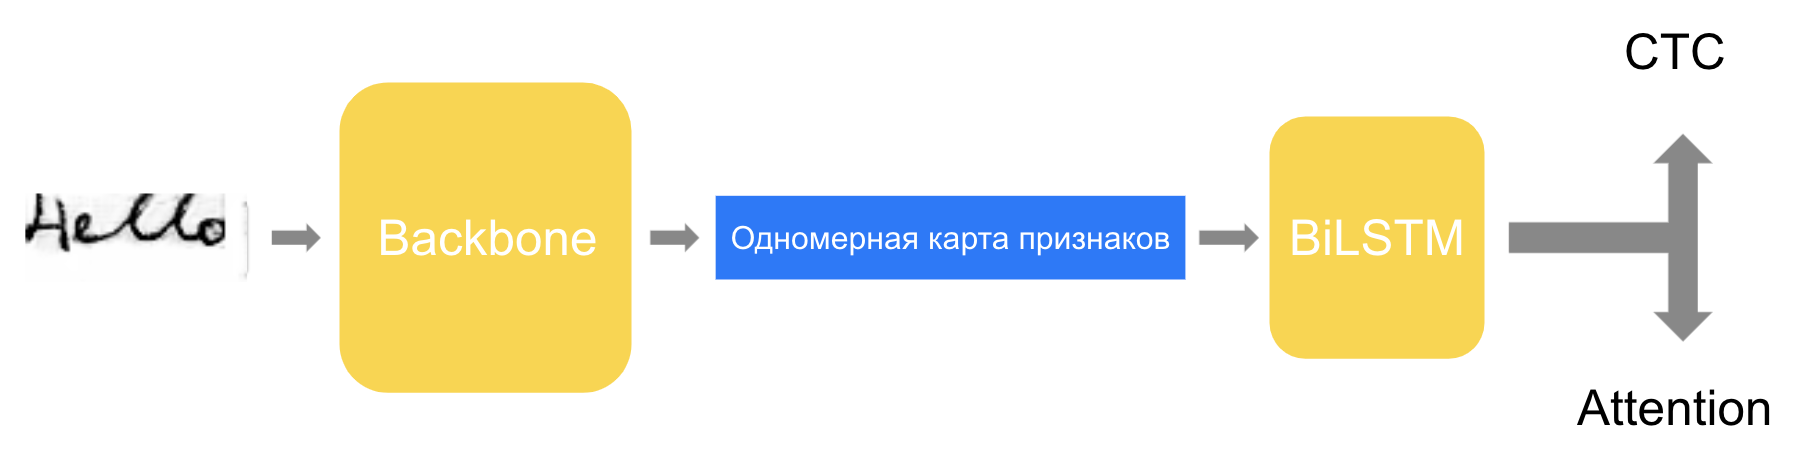
\includegraphics[width=\linewidth]{recognition.png}
    \caption{Стандартная модель распознавания}
    \label{standard_recognizer}
\end{figure}

Современные модели распознавания текстов построены по похожим принципам. Разберем некоторые особенности на примере модели, 
которую мы будем использовать в качестве основной в данной работе.
На Рис.\ref{standard_recognizer}  изображена стандартная архитектура нейросети для распознавания. Разберем основные особенности:

\begin{itemize}
    \item На вход подается изображение с заранее неизвестной шириной
    \item Backbone -- это любая нейросеть, умеющая извлекать высокоуровневые признаки из картинки. Обычно используются
    модели, обученные на ImageNet
    \item На выходе из backbone получаем одномерную карту признаков -- изображение с большим количеством каналов, высотой h=1px
    и шириной зависящей от входного изображения
    \item Т.к. мы считаем, что в тексте символы сильно связаны необходимо привнести в полученную карту признаков некоторые нелокальные
    зависимости. В нашей архитектуре этого можно добиться, используя BiLSTM.
    \item На выходе из BiLSTM мы получаем одномерную карту признаков того же размера, но с учтенными нелокальными зависимостями.
    \item Для преобразования карты признаков в текст можно использовать рекуррентую нейросеть с вниманием, либо CTC loss,
    часто использующийся в OCR

\end{itemize}


\subsection{Метрики}

Для понимания качества распознанного текста используются нетривиальные техники подсчета качества.
Они делятся на два вида: пословные, посимвольные. Отличие состоит в том, что мы считаем минимальной сущностью (токеном),
которая может быть правильной и неправильной при предсказании. На уровне слов ошибка в одном символе приведет
к ошибке на всем слове, на уровне символов ошибка -- это неправильный символ на некоторой позиции.
Ошибки бывают трех типов: ошибка в токене, пропуск токена, лишний токен. Для того, чтобы верно учитывать ошибки,
связанные с пропуском/добавлением токена необходимо ''выровнять'' предсказанный текст до верного. Для этого запустим
запустить процедуру поиска расстояния Левенштейна, которая вернет количество вставок, удалений и замен. 
Выделяют две основных метрики: word error rate (WER), character error rate (CER)\footnote{Заметим, что эти метрики могут быть больше 1}

\newpage


$$CER = \frac{S_c + D_c + I_c}{N_c}$$

$$WER = \frac{S_w + D_w + I_w}{N_w}$$

где $S_{*}$ -- количество замен, $I_{*}$ -- количество вставок, $D_{*}$ -- количество удалений


\subsection{Генерация синтетических изображений}

\begin{figure}[htb]
    \centering
    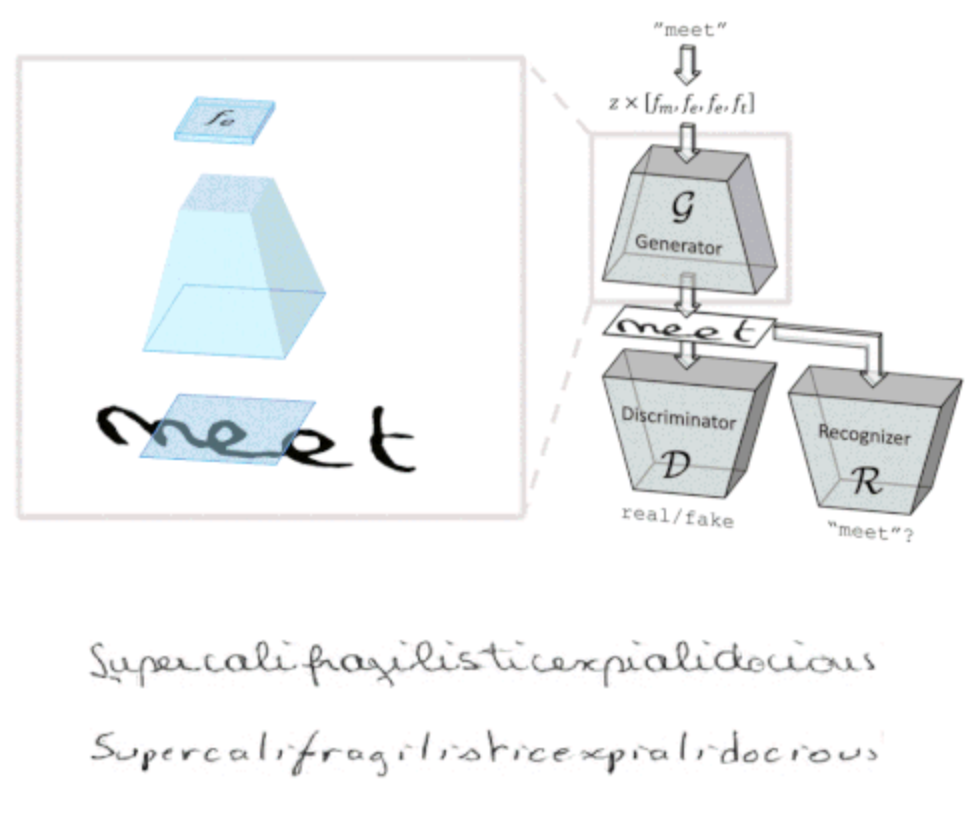
\includegraphics[width=0.6\linewidth]{scrabble_gan.png}
    \captionof{figure}{Scrabble Gan}
    \label{fig:gan}
\end{figure}


Для генерации синтетических изображений рукописного текста использовалась архитектура Scrabble Gan \cite{scrabble_gan}.

\vspace{10pt}
Данная модель состоит из трех частей:
\begin{itemize}
    \item Генератор -- полностью сверточная нейросеть, использующая  транспонированные свертки для получения конечного изображения
    из  бинарных векторов соответствующих символам алфавита.
    \item Дискриминатор, который ''исследует'' изображение в целом и относит  изображение к ''подделка'', ''реальные данные''
    \item Распознаватель, который ''читает'', что написано на картинке и сравнивает с эталоном.
\end{itemize}

\section{Этапы работы}

Цель всей работы состоит в обучении модели распознавания рукописного текста на русском и английском языке. Для
этого необходимы данные для обучения. В случае английского языка можно использовать IAM dataset \cite{iam}, для 
русского языка существует датасет CyrHD, но он не подходит под специфику коммерческого использования.
Данный датасет преимущественно состоит из слов, не не из линий/строк текста, что автоматически делает его менее полезным
для реального использования. Поэтому было решено начать сбор своего датасета.

\subsection{Сбор данных}

Сбор данных проводился через краудфандинг сервис ''Толока''. 

\vspace{10pt}

\begin{figure}[htb]
    \centering
    \begin{minipage}{.55\textwidth}
        \centering
        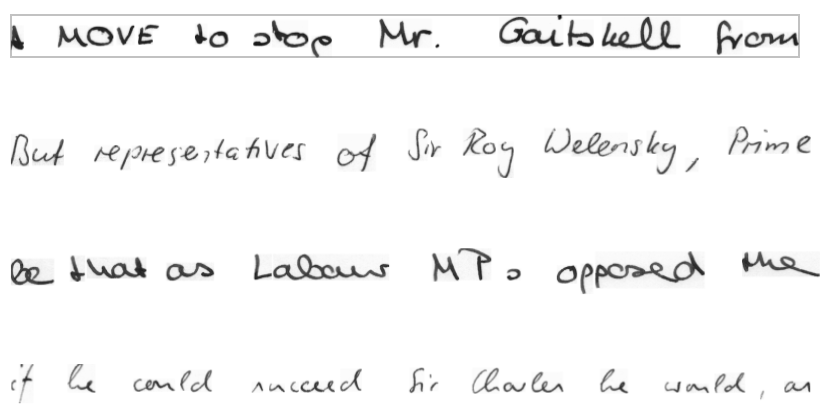
\includegraphics[width=\linewidth]{IAM.png}
        \captionof{figure}{IAM}
        \label{fig:IAM}
    \end{minipage}%
    \begin{minipage}{.45\textwidth}
        \centering
        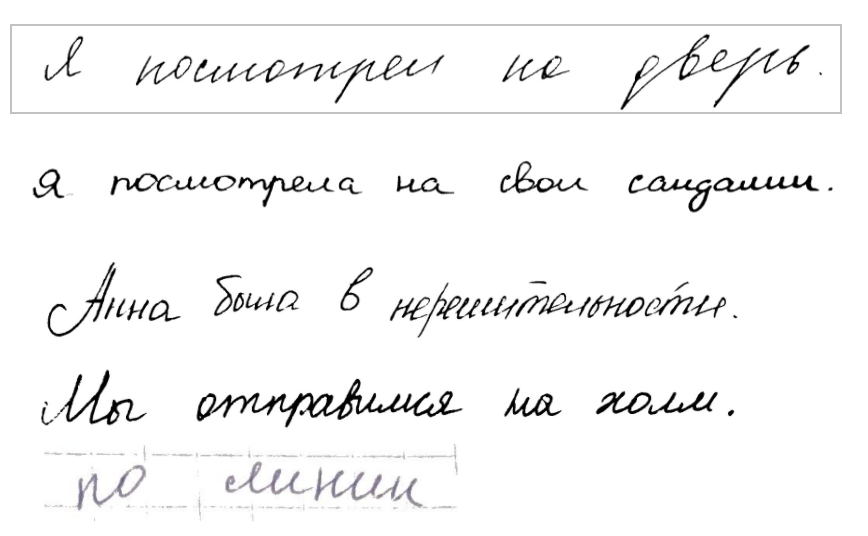
\includegraphics[width=\linewidth]{RHD.png}
        \captionof{figure}{RHD (ours)}
        \label{fig:RHD}
    \end{minipage}
\end{figure}

Сбор данных делился на следующие этапы:
\begin{itemize}
    \item Создание/сбор текстов для задания ''написать и сфотографировать текст''
    \item Люди пишут и фотографируют заранее заданную строку текста, которая выбирается из 
    собранных данных на предыдущем этапе
    \item Другие люди проверяют изображение на соответствие некоторым критериям
    \item Строки текста извлекаются с помощью детектора, обученного на печатных текстах. 
    Данный детектор хорошо работает и в случае рукописных текстов.
\end{itemize}

\subsection{Аугментация}

В случае рукописных текстов нельзя не воспользоваться искусственным методом увеличения выборки -- агументацией.

\begin{figure}[htb]
    \centering
    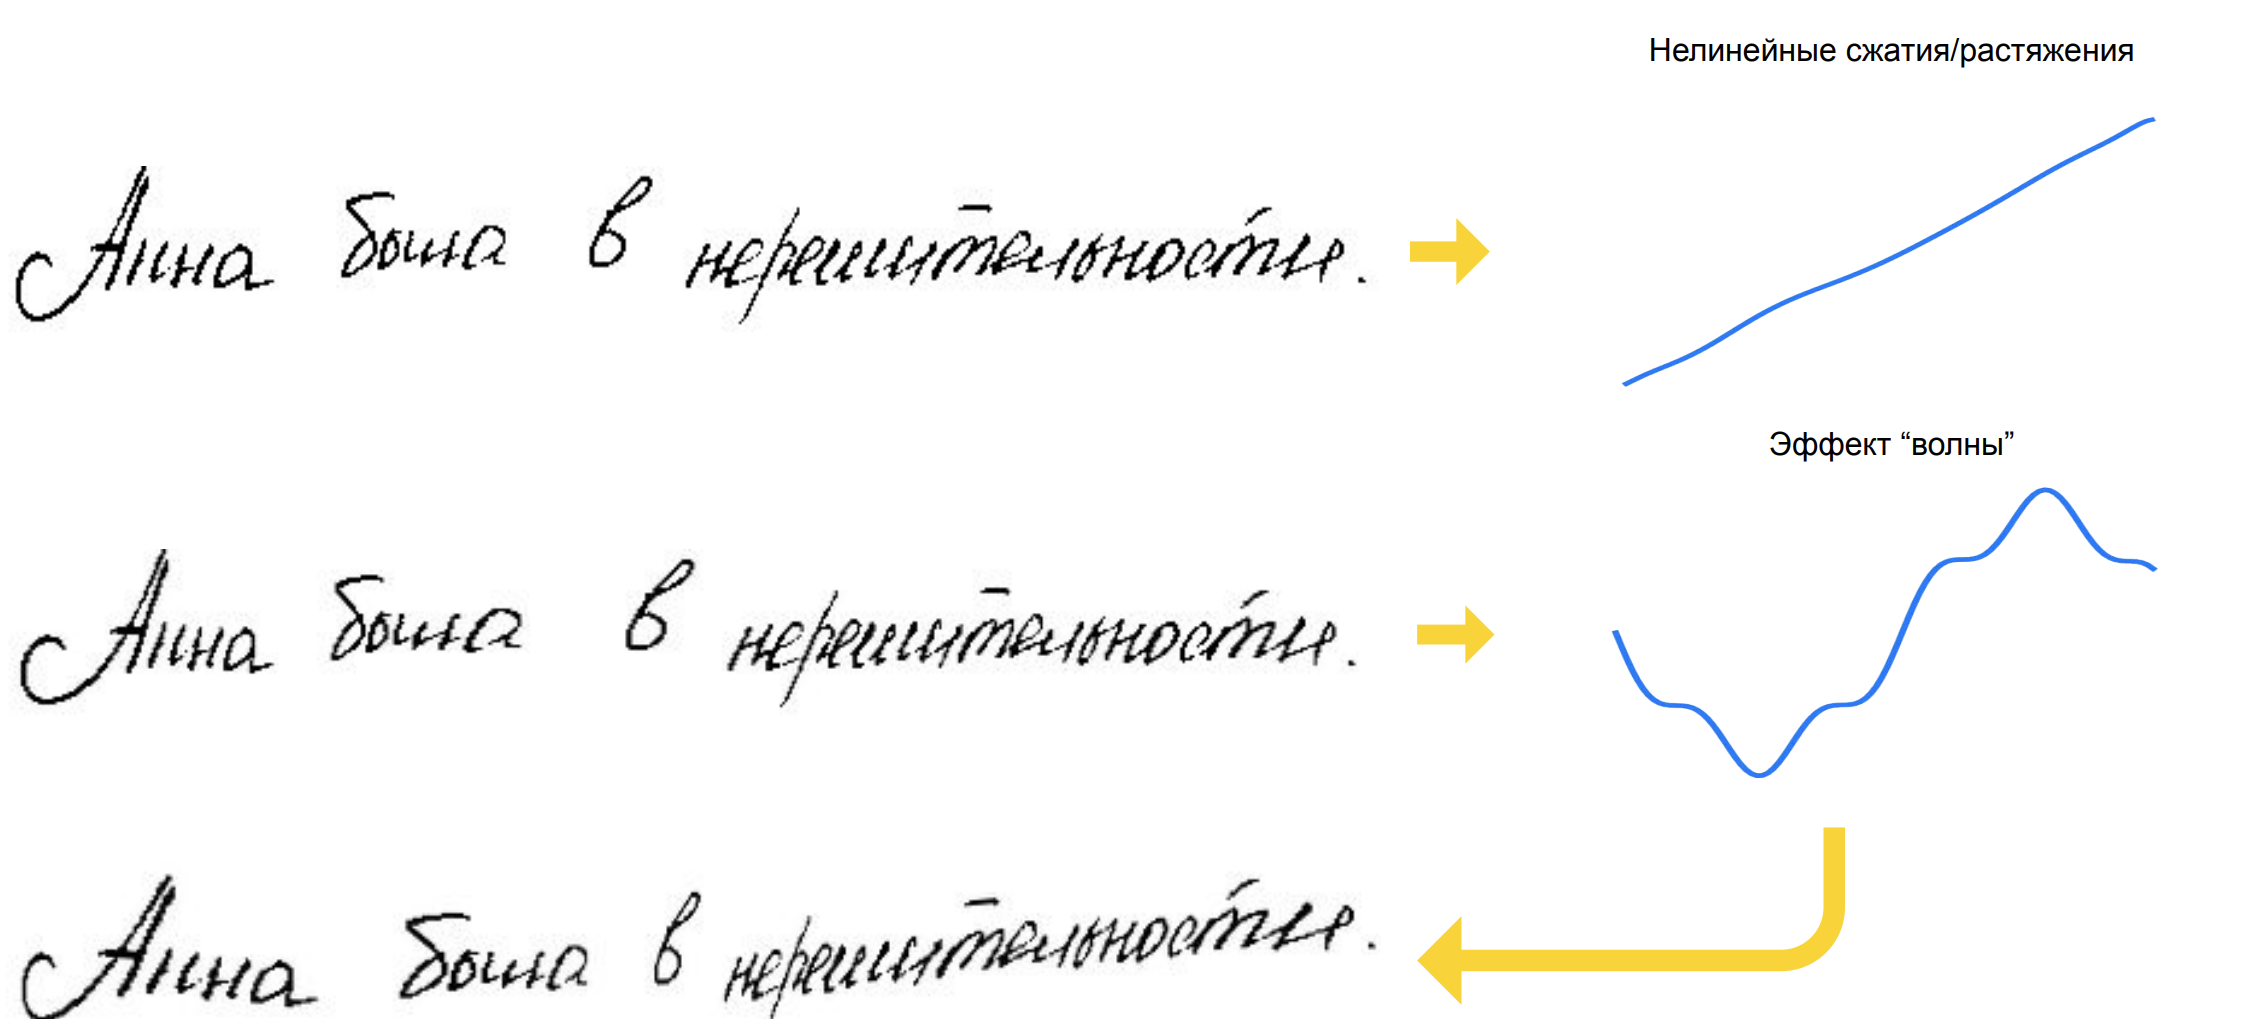
\includegraphics[width=\linewidth]{aug.png}
    \captionof{figure}{Augmentation}
    \label{fig:aug}
\end{figure}

Были разработаны два вида аугментации (Рис.\ref{fig:aug}):

\begin{itemize}
    \item Нелинейные сжатия/растяжения -- каждая точка изображения сдвигается по координате X на некоторое расстояние от своего изначального положения.
    \item Эффект ''волны'' -- каждая точка изображения сдвигается по координате Y на некоторое расстояние.
\end{itemize}

\subsection{''Рукописные'' шрифты}

В виду легкой доступности генерации ситнетических печатных текстов было решено попробовать сгенерировать тексты,
использующие шрифты, похожие на рукописные (Риc.\ref{fig:fonts})

\begin{figure}[htb]
    \centering
    \begin{minipage}{.5\textwidth}
        \centering
        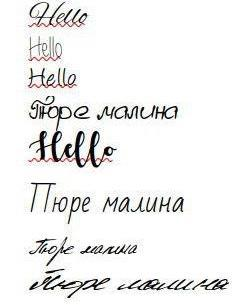
\includegraphics[width=0.5\linewidth]{pure_malina.jpg}
    \end{minipage}%
    \begin{minipage}{.5\textwidth}
        \centering
        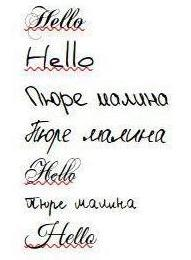
\includegraphics[width=0.5\linewidth]{pure_malina_1.jpeg}
    \end{minipage}
    \caption{''Рукописные'' шрифты}
    \label{fig:fonts}
\end{figure}



\subsection{Эксперименты}

\subsubsection{IAM}



\begin{figure}[htb]
    \centering
    \begin{minipage}{.45\textwidth}
        \centering
        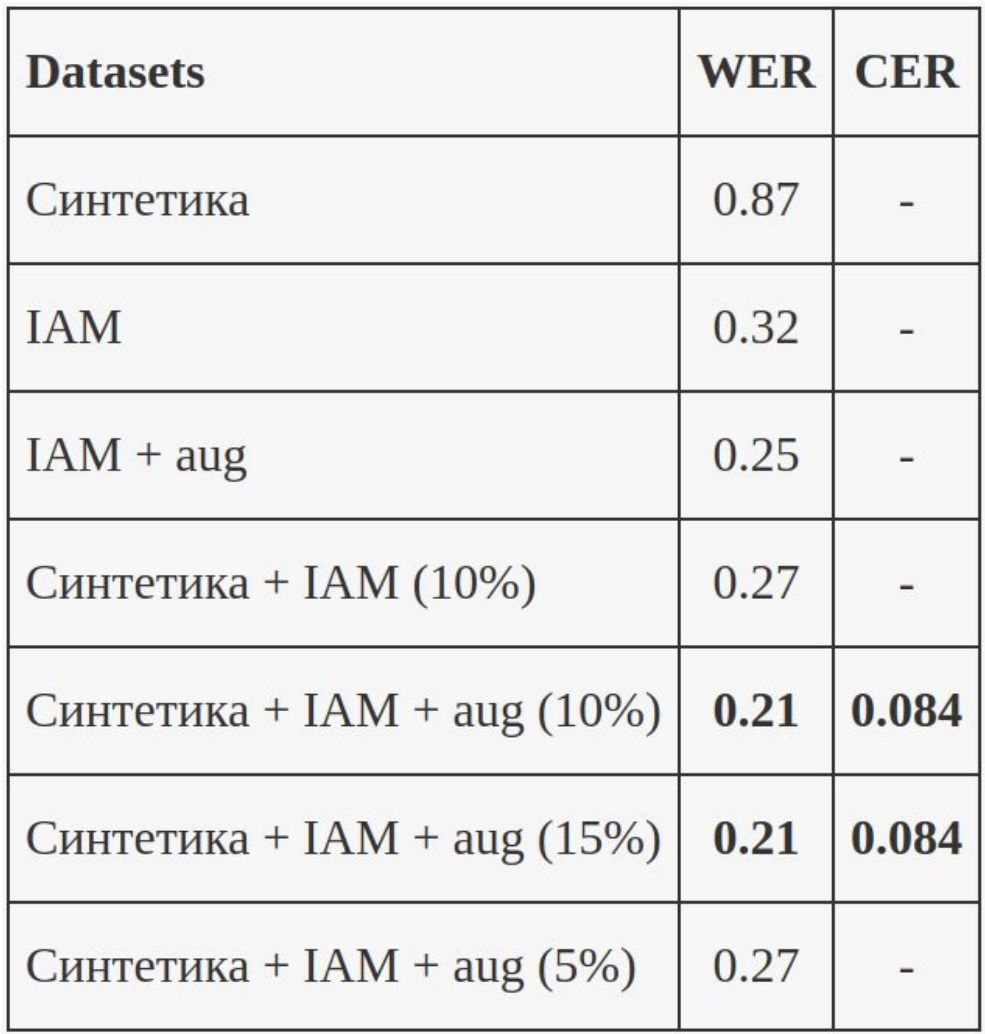
\includegraphics[width=0.65\linewidth]{IAM_compare.png}
        \captionof{table}{Сравнение качества нашей модели на разных данных}
        \label{table:compare_iam}
    \end{minipage}%
    \begin{minipage}{.55\textwidth}
        \centering
        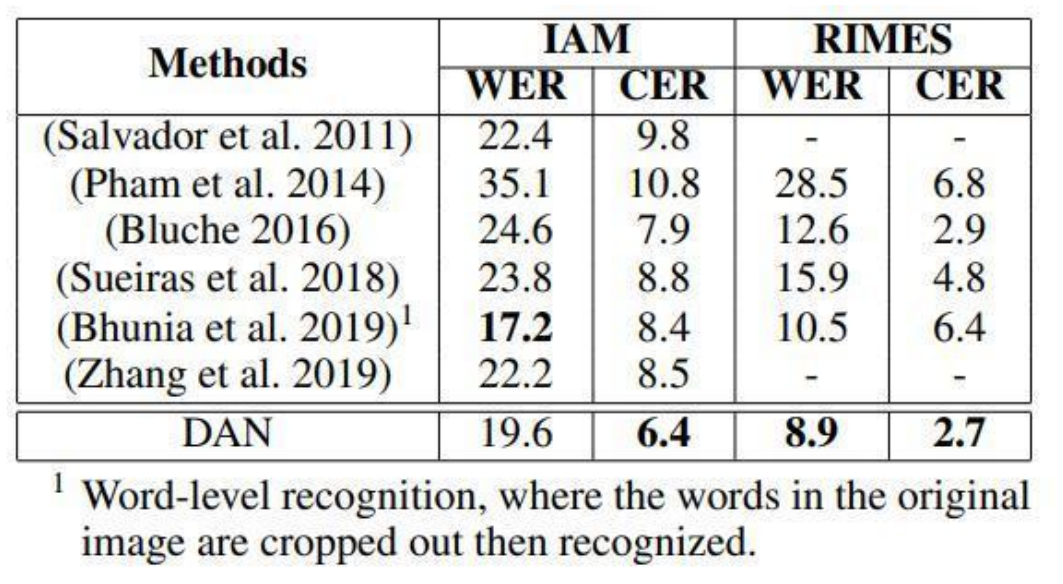
\includegraphics[width=\linewidth]{iam_compare_dan.png}
        \captionof{table}{Предыдущие работы}
        \label{table:compare_iam_dan}
    \end{minipage}
\end{figure}


В Таб.\ref{table:compare_iam} представлены результаты экспериментов для разных соотношениях
синтетических данных, исходного IAM, аугментированного IAM.
Модель, обученная на полностью  синтетических данных, как и ожидалось показала плохие результаты.
Эксперименты с IAM без аугментаций дают результаты существенно 
лучше, чем чистая синтетика. Добавление аугментации улучшило качество еще на 7\%. 
Наиболее успешной конфигурацией оказалась синтетика  в сочетании с агументированным IAM

В Таб.\ref{table:compare_iam_dan} агрегированы результаты некоторых статей. Можно видеть, что в сравнении наша модель
занимает 2-ое место\footnote{Bhunia er al. 2019 в расчет не берется, они сами вырезали строки текста из исходного датасета} по метрике WER,
что можно считать очень хорошим результатом, учитывая, что мы не отходили от стандартной архитектуры модели.

\subsubsection{Русскоязычные датасеты}

\begin{figure}[htb]
    \centering
    \begin{minipage}{.45\textwidth}
        \centering
        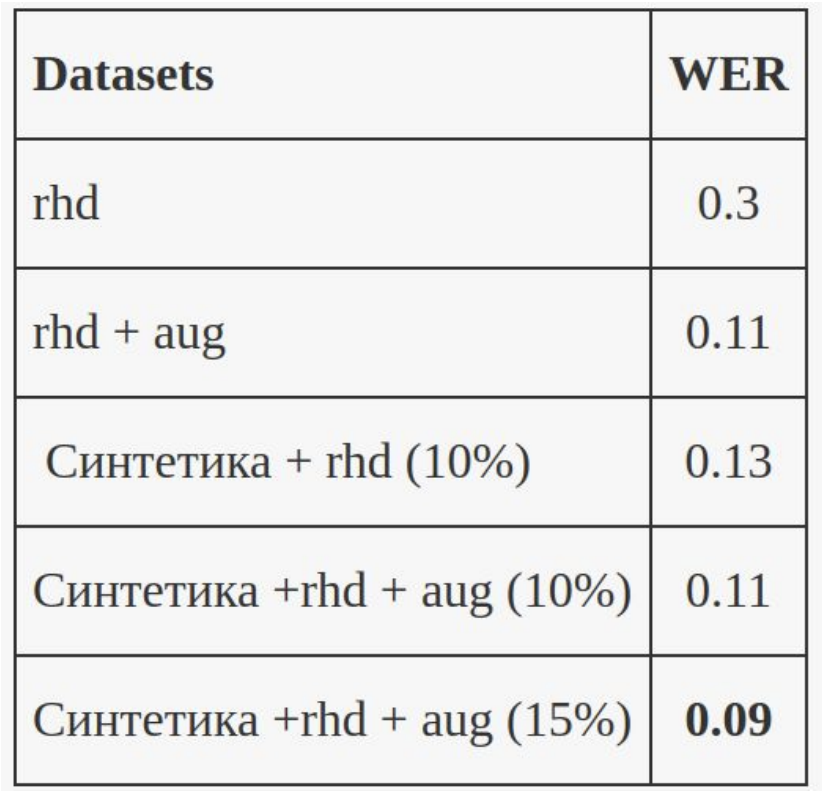
\includegraphics[width=0.65\linewidth]{rhd_compare.png}
        \captionof{table}{Сравнение качества нашей модели на разных данных}
        \label{table:rhd_compare}
    \end{minipage}%
    \begin{minipage}{.55\textwidth}
        \centering
        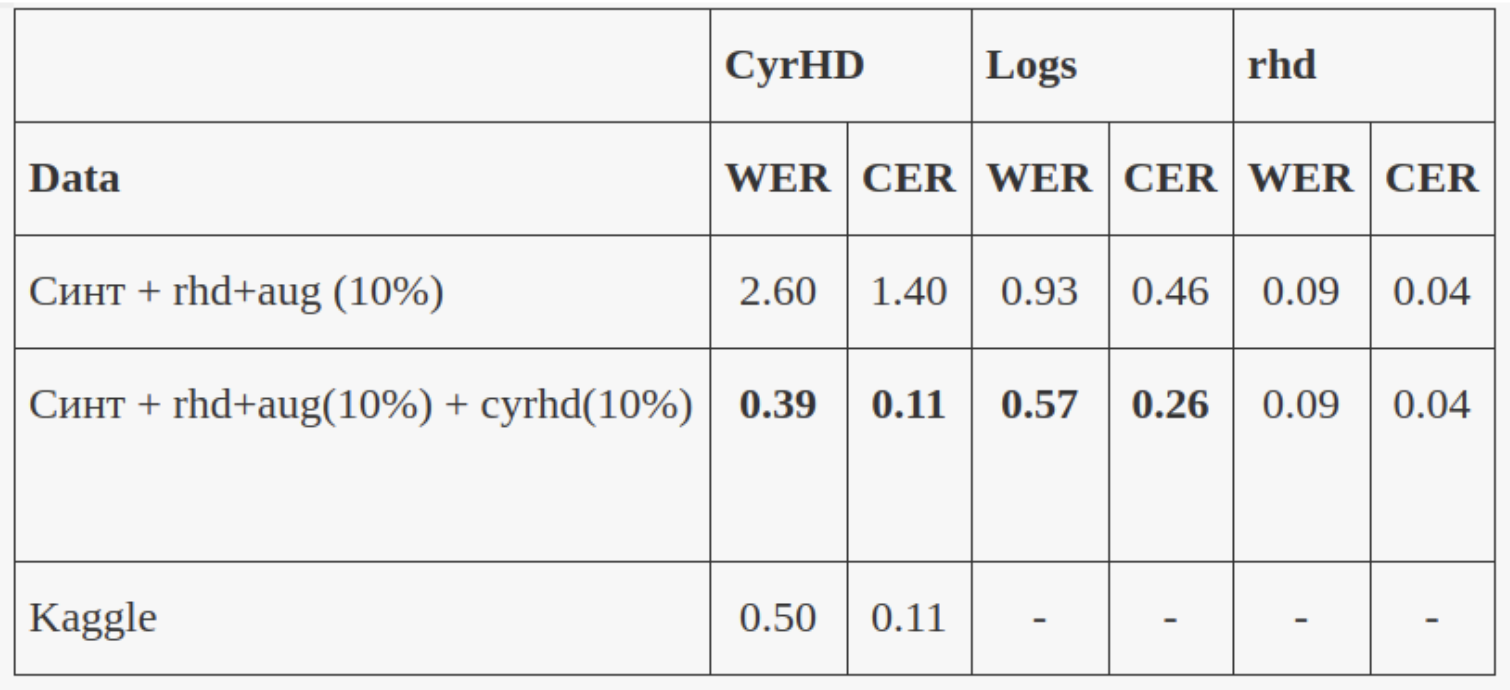
\includegraphics[width=\linewidth]{russ_compare.png}
        \captionof{table}{Предыдущие работы}
        \label{table:russ_compare}
    \end{minipage}
\end{figure}

В Таб. \ref{table:rhd_compare} представлены результаты экспериментов для разных соотношениях
исходного RHD, аугментированного RHD.
Эксперименты с RHD без аугментаций дают результаты неплохой результат,
но добавление аугментации разительно улучшает качество на 19\%.
Наиболее успешной конфигурацией оказалась синтетика  в сочетании с аугментированным IAM

В Таб. \ref{table:russ_compare} в столбце CyrHD можно сравнить качество нашей модели с лучшим решением
с платформы Kaggle. Нам удалось улучшить качество по метрике WER на 10\%, получив значение 0.39.


\subsection{Генерация изображений}
\begin{figure}[htb]
    \centering
    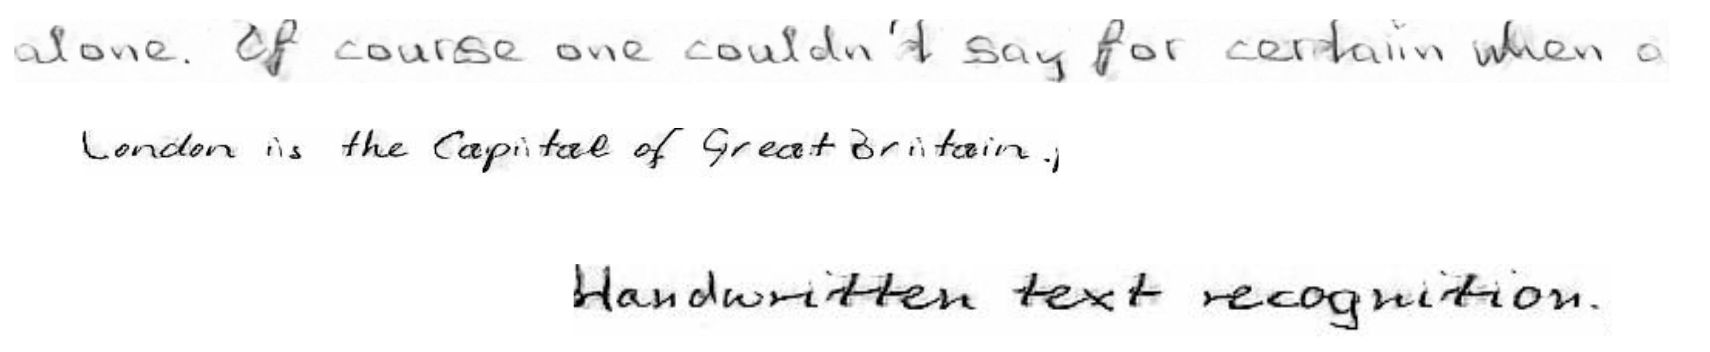
\includegraphics[width=\linewidth]{english_gan.png}
    \captionof{figure}{Примеры сгенерированных изображений на английском языке}
    \label{fig:english_gan}
\end{figure}
Для генерации английского языка был обучен Scabble GAN на датасете IAM. Нам удалось восстановить результаты
из статьи и получить рукописные тексты приемлемого качества


\begin{figure}[htb]
    \centering
    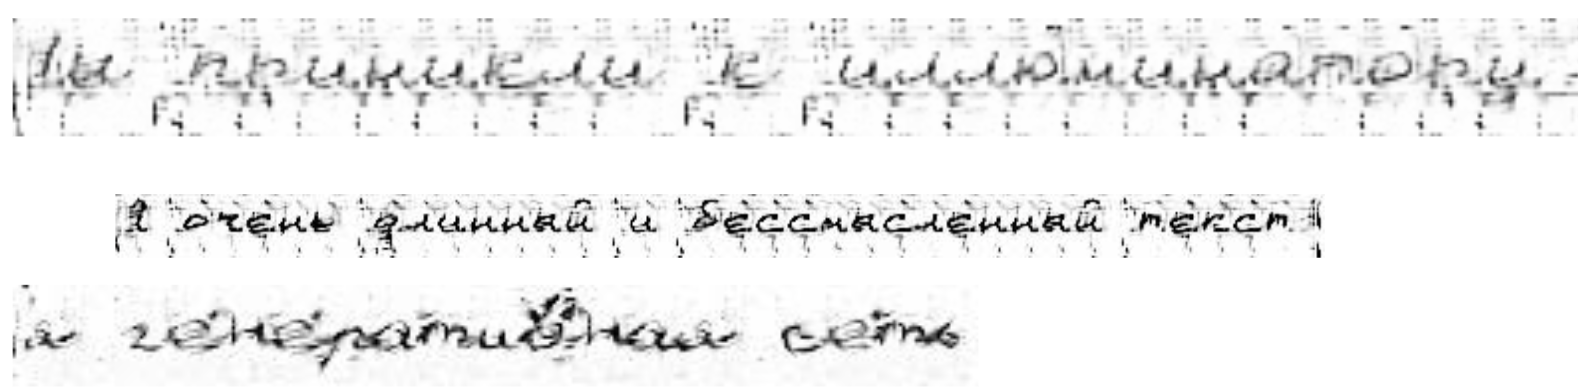
\includegraphics[width=\linewidth]{russian_gan.png}
    \captionof{figure}{Примеры сгенерированных изображений на русском языке}
    \label{fig:english_gan}
\end{figure}
Для генерации русского языка был обучен Scabble GAN на датасете RHD.
Нам не удалось получить приемлемое качество для русского языка. Одной из причин может служить семантическая простота 
нашего датасета -- текст часто был достаточно прост и предсказуем, поэтому
распознаватель мог переобучиться под него. Также русский рукописный текст субъективно более сложен для написания,
в нем присутствуют нетривиальные связи между буквами в отличии от английского языка, где таких связей меньше.


\section{Заключение}
В данной работе был собран большой датасет русского рукописного текста, обучена модель на английском языке показывающая качество,
сравнимое с лучшими моделями, обучена модель на русском языке, а также исследовано поведение генеративной сети Scrabble Gan для 
генерации русского рукописного текста.

\newpage
\begin{thebibliography}{9}
    \bibitem{CNN-BGRU}
    Abdallah A., Hamada M., Nurseitov D.
    Attention-based Fully Gated CNN-BGRU for Russian Handwritten Text //Journal of Imaging. – 2020. – Т. 6. – №. 12. – С. 141.

    \bibitem{scrabble_gan}
    Fogel S. et al. Scrabblegan: Semi-supervised varying length handwritten
    text generation //Proceedings of the IEEE/CVF Conference on 
    Computer Vision and Pattern Recognition. – 2020. – С. 4324-4333.

    \bibitem{dan}
    Wang T. et al. Decoupled attention network for text recognition 
    //Proceedings of the AAAI Conference on Artificial Intelligence. – 2020. – Т. 34. – №. 07. – С. 12216-12224.

    \bibitem{chd}
    www.kaggle.com/constantinwerner/cyrillic-handwriting-dataset

    \bibitem{hkr}
    github.com/abdoelsayed2016/HKR\_Dataset

    \bibitem{iam}
    https://fki.tic.heia-fr.ch/databases/iam-handwriting-database

\end{thebibliography}

\end{document}